\begin{tikzpicture}[/pgf/declare function={f=sin(deg(0.5*pi*x+0.25*pi));g=sin(deg(pi*x));}]
\begin{axis}[
    width=\textwidth,
    height=0.6\textheight,
    domain=0:10,
    samples=500,
    axis lines=middle,
    xticklabel=$t_{\pgfmathprintnumber{\tick}}$
]
\addplot [dashed, thick] {f};
\addplot [red, thick] {g};
    \addplot [mark=*, only marks] coordinates {(0.5,1) (4.5, 1) (8.5,1) (1.83, -0.5) (3.16,-0.5) (5.83,-0.5) (7.16,-0.5) (9.83,-0.5)};
\end{axis}
\end{tikzpicture}
